\documentclass{article}

\usepackage[english]{babel}

\usepackage{amsmath}
\usepackage{amsthm}
\usepackage{amssymb}
\usepackage{mathtools}
\usepackage{siunitx}
\usepackage{float}
\usepackage[thinc]{esdiff}
\usepackage{tikz}
\usepackage{pgfplots}
\usepackage{booktabs}
\usepackage{minted}

\usepackage[pdfborderstyle={/S/U/W 0}]{hyperref}

\newtheorem{theorem}{Theorem}
\newtheorem{lemma}[theorem]{Lemma}
\newtheorem{prop}{Proposition}

\DeclareMathOperator*{\argmax}{arg\,max}
\DeclareMathOperator*{\argmin}{arg\,min}

\begin{document}

\section{Generating data}

\subsection{Intro}

The cost function, in function of departure time \(t_d\), is
\begin{equation}
  \label{eq:cost_td}
  C(t_d) = \alpha tt(t_d) + \beta[t^*-t_d-tt(t_d)]^+ + \gamma[t_d+tt(t_d)-t^*]^+ 
\end{equation}
where
\begin{itemize}
\item \(t^*\) is the desired arrival time
\item \(\alpha\) is the value of time spent travelling
\item \(\beta\) is the value of time spent waiting there
\item \(\gamma\) is the value of time arriving late
\item \(tt(t_d)\) is the time spent travelling if leaving at time \(t_d\)
\item \([x]^+ = \max(0, x)\)
\end{itemize}

\subsection{Are $t_a$ and $t_d$ equivalent?}

It would be helpful to express the cost function in term of the arrival time \(t_a = t_d + tt(t_d)\),
so that the second part of the cost function would greatly simplify
\[ \beta[t^*-t_d-tt(t_d)]^+ + \gamma[t_d+tt(t_d)-t^*]^+ = \beta[t^*-t_a]^+ + \gamma[t_a-t^*]^+ \]

But how do we express the first term \(tt(t_d)\) in terms of \(t_a\)?

\begin{equation}
  \label{eq:ta_td}
  t_a(t_d) = t_d + tt(t_d)
\end{equation}

Note that the travel time can be expressed in terms of the arrival time \(t_a\) if and only if the function
\eqref{eq:ta_td} is invertible:
this is because the departure time can be easily reconstructed from the travel time and the arrival time (and viceversa).

\subsubsection{When are they equivalent?}

Inverting \eqref{eq:ta_td} is not analytically possible a priori, and may not be possible in general.
It only depends on whether the function \(-tt(t_d)\) ever grows more than the identity.
For instance, if the travel time is a gausssian
\begin{equation*}
  tt(t_d) = \frac{1}{\sigma\sqrt{2\pi}}\exp\left(-{\frac{t_d^2}{2\sigma^2}}\right)
\end{equation*}
then the arrival time is invertible if and only if the variance \(\sigma\) satisfies the condition
\[\sigma \geq (2\pi e)^{-\frac{1}{4}} \approx 0.492 \]

In general, assuming that the function grows less than the identity is pretty reasonable,
since in real world I think leaving later results in arriving later.

From now on, assume \eqref{eq:ta_td} is invertible, and \(tt_a(t_a) = tt(t_d(t_a))\) exists.
Moreover, \(\alpha = 1\).

\subsection{Where is the cost minimized?}

\begin{equation}
  \label{eq:cost_ta}
  C(t_a) = tt_a(t_a) + \beta[t^*-t_a]^+ + \gamma[t_a-t^*]^+
\end{equation}

The cost function \eqref{eq:cost_ta} could be minimized either at the only non differentiable point (for \(t_a = t^*\))
or at one of the points where its derivative is zero.
\begin{equation}
  \label{eq:cost_diff}
  C'(t_a) =
  \begin{cases}
    tt_a'(t_a) -\beta \quad &\text{if } t_a < t^* \\
    tt_a'(t_a) + \gamma \quad &\text{otherwise}
  \end{cases}
\end{equation}

Setting it equal to zero, the minimum is realized by one of the points

\begin{align*}
  & t_a |\ tt_a'(t_a) = \beta, t_a < t^* \\
  & t_a = t^* \\
  & t_a |\ tt_a'(t_a) = -\gamma, t_a > t^* \\
\end{align*}

\subsubsection{If travel time is 1-lipschitz then we have at most 2 minima}

Note that, here, assuming

\begin{equation}
  \label{eq:cond_late_min}
|tt_a'(t_a)| < 1 \ \forall t_a, \qquad \gamma > \alpha = 1
\end{equation}
implies that there is no time that satisfies the last condition, that means that arriving late never realises a (not even local) minimum.

These assumptions are reasonable for what discussed earlier, but \textcolor{red}{this should be looked at better}.

\textcolor{green}{I looked at it better!} Here is the results

\subsubsection{We don't need travel time to be 1-lipschitz, in general we have 3 minima}

This is because we only need \(tt(t_d)\) to decrease slower than \(-x\), and this will make \(tt_a(t_a)\) never increase more than \(x\).

Consider indeed

\begin{align*}
  t_a(t_d) & = t_d + tt(t_d)
\end{align*}

This yields
\begin{equation*}
  tt_a(t_a) = tt(t_a^{-1}(t_a))
\end{equation*}
differentiating,
\begin{align*}
  \diffp{tt_a(t_a)}{{t_a}} & = tt'(t_a^{-1}(t_a)) \diffp{t_a^{-1}(t_a)}{{t_a}} \\
  & = tt'(t_a^{-1}(t_a)) \frac{1}{t_a'(t_a^{-1}(t_a))}
\end{align*}

But we know that \(t_a'(t_d) = 1 + tt'(t_d)\).

This implies
\begin{align*}
  \diffp{tt_a(t_a)}{{t_a}} & = tt'(t_d) \frac{1}{1+tt'(t_d)} \\
  & = \frac{tt'(t_d)}{1+tt'(t_d)} < 1
\end{align*}

\subsubsection{Gaussian travel time}

Again, let's look at the case in which the travel time is gaussian.
I assume that the travel time is gaussian in function of the arrival time as well,
and this can be justified by saying that
\[t_a - t_d >> \max_t | tt'(t)|\]
but \textcolor{red}{I doubt that this is an assumption that can be made}.
Still, assume that
\begin{equation}
  \label{eq:travel_time_gauss}
  tt_a(t_a) = \frac{1}{\sigma\sqrt{2\pi}}\exp\left(-{\frac{t_a^2}{2\sigma^2}}\right)
\end{equation}
and so
\begin{equation}
  \label{eq:travel_time_gauss_diff}
  tt_a'(t_a) = -\frac{t_a}{\sigma^3\sqrt{2\pi}}\exp\left(-{\frac{t_a^2}{2\sigma^2}}\right)
\end{equation}
This can't be inverted analytically and the solutions to the equations above can be found numerically.
(I hope other approaches for minimizing the cost are possible, but nothing comes to my mind right now).

\subsubsection{In general, how to find the minima}


In order to find the minimum of the function \(C(t_a)\) there are thus two possible procedures (that are actually the same one...).
\begin{itemize}
\item Running a root finding algorithm on the functions \(tt_a'(t_a) - \beta,\ tt_a'(t_a) + \gamma\) to find at most two local minima, to be compared to the one potentially realized by \(t^*\) to find the minimum
\item Directly running an optimizer on the cost function \(C(t_a)\). This would find one of the local minima.
  Initializing two optimizers for a very high value and a very low value would find the two minima found above.
  Moreover, in the case in which conditions \eqref{eq:cond_late_min} hold,
  it is enough to launch one optimizer for a very little value.
  This could be the best way, since it is simpler and equally effective (and potentially delegates the computation of an explicit expression for \(tt'\) to an automatic differentiation framework).
\end{itemize}

I will thus implement the second point.

\textcolor{blue}{The second point is not working too well due to (appearently) some problems with jaxopt.GradientDescent. Maybe implementing the first one is actually not a bad idea.}

\section{Is the optimum monotonous in $t^*$?}

\subsection{If travel time is 1-Lipschitz}

In particular, let's again assume the travel time to be 1-Lipschitz (so that the minimum of the cost function can never be realized by \(t > t^*\)), and \(C^1(\mathbb{R})\)
on top of going asymptotically to zero as the arrival time goes to \(\infty\) and \(-\infty\).

As discussed earlier, the cost will be minimized either for a point for which \(tt_a'(t_a) = \beta\) or for \(t_a = t^*\).

Consider thus the sets
\begin{align*}
  B & = \{t_a | tt_a'(t_a) = \beta, tt_a'' > 0\} \\
  B_{t^*}&  = \{t_a | tt_a'(t_a) = \beta, t_a \leq t^*\}
\end{align*}

\subsubsection{Where the travel time function is increasing}

First of all, consider the intervals in which the travel time function \(tt_a\) is increasing.

Here, new potential optima can be created.
The following lemma shows that every time a potential optimum is created (when the set \(B_{t^*} \) grows), the function will locally be constant.

\begin{lemma}
  Let \(t_b \in B\). Then, \(\exists \delta > 0 |\ t_a(t^*) = t_b \ \forall t^* \in [t_b, t_b + \delta)\)
\end{lemma}
\begin{proof}
  Let \(t_0 = t_b + \epsilon\), such that \(tt'(t) > \beta\ \forall\ t \in (t_b, t_0)\).

  The function to be minimized will be
  \begin{equation*}
    C[t^* = t_0](t_a) = tt_a(t_a) + \beta(t_0 - t_a)
  \end{equation*}
  and will be minimized either for \(t_a = t_0\) or for \(t_a = t_b\).

  But, since the derivative is lower bounded,

  \begin{align*}
    C[t^*=t_0](t_0) & = tt_a(t_0) \\
    & = tt_a(t_b + \epsilon) \\
    & = tt_a(t_b) + \int_{t_b}^{t_0} tt'(t) dt \\
    & \geq tt_a(t_b) + \beta(t_0 - t_b) \\
    & = C[t^* = t_0](t_b)
  \end{align*}

  The minimum is thus constant for each admissible value of \(\epsilon\), and such an epsilon can be chosen by continuity of the function \(tt_a'\).
\end{proof}

The following lemma shows that the function can never \textit{jump back}:

\begin{lemma}
  Let \(t_b \in B\), \(t_0 > t_b\) such that \(t_a(t_0) = t_0\).
  
  Then, \(\nexists t_1 > t_0 |\ t_a(t_1) = t_b\),
\end{lemma}
\begin{proof}
  There are two cases: either \(tt_a'(t_0) \geq \beta\) or \(tt_a'(t_0) < \beta\).

  If  \(tt_a'(t_0) < \beta\), then the minimum realized  by \(t_0\) is growing slower than the minimum realized by \(t_a\): we can reduce \(t_0\), until we fall in the other case. We must fall in the other case, since \(t_b \in B\)

  If \(tt_a'(t_0) \geq \beta\), it is impossible that the hypothesis \(t_a(t_0) = t_0\) is satisfied:
  each time that \(tt_a'(t_0) \geq \beta\), for what said earlier the function is constant, and not linear.
\end{proof}

As long as the function \(tt\) is increasing, the only admissible jumps are upwards (from a constant function to the identity).

\subsubsection{Where the travel time function is decreasing}

Where the function is decreasing, no new candidates for the minima are possible, since \(\beta > 0\).

If \(t_a(t) = t\), then as long as the function \(tt\) is decreasing the optimal time will grow linearly.

Otherwise, if \(t_a(t) = t_b \neq t\), then the function will remain constant until \(tt_a(t) = \beta (t - t_b)\),
and then jump and grow, again, as the identity.

\subsection{In general}

Consider now an arbitrary travel time function \(tt_a(t_a)\).

Consider the sets

\begin{align*}
  B & = \{t_a | tt_a'(t_a) = \beta, tt_a'' > 0\} \\
  G & = \{t_a | tt_a'(t_a) = -\gamma, tt_a'' > 0\} \\
\end{align*}

The function \(t_a(t^*)\) is (locally) either equal to the identity \(t_a(t^*) = t^*\) or constant, assuming a value that is in one of the defined sets \(B, G\)

\begin{prop}
  Let \(tt_a(t_a)\) be a travel time function with only one local maximum \(\hat{t}\),
  and let (in increasing order) \(B = \{b_1, \dots, b_n\}\), \(G = \{g_1, \dots, g_m\}\).


  Consider the collections of intervals \(B^* = \{(b_i, f(b_i))\}_i\) and \(G^* = \{(h(g_i), g_i)\}_i\), where
  
  \begin{align*}
    f(t) & = \min\{x>t | \int_t^x(tt_a(s) - tt_a(t)) ds = 0\} \\
    h(t) & = \max\{x<t | \int_x^t(tt_a(s) + tt_a(t)) ds = 0\} \\
  \end{align*}

  If \(f(b_n) \leq g(g_1)\), then the function \(t_a(t^*)\) will be as follows:

  \begin{align*}
    t_a(t^*) = 
    \begin{cases}
      \min \{b_i | t^* \in (b_i, f(b_i))\} & \text{if } \exists i |\ b_i < t^* < f(b_i) \\
      \max \{g_i | t^* \in (h(g_i), g_i)\} & \text{if } \exists i |\ h(g_i) < t^* < g_i \\
      t^* & \text{otherwise}
    \end{cases}
  \end{align*}

  Otherwise, if \(f(b_n) > g(g_1)\), for \(f(b_n) < t^* < h(g_1)\) the function will be made by an increasing succession of constant zones.
\end{prop}

\section{Retrieving parameters}

\subsection{Intro}

For retrieving the parameters from the data, I will try to define a function that,
given the distribution of the parameters, estimates the likelihood of each point.

For this, it is probably a good idea to use the characterization of the function \(t_a(t^*)\) above.

From now on,
\begin{equation*}
  ot(t) := t_a(t)
\end{equation*}

Let \(t_a\) be a sample of the optimal arrival time. The likelihood of the parameters will be
\begin{equation}
  \label{eq:likelihood_def}
  \mathcal{L}(\mu_\beta, \mu_\gamma, \mu_t, \sigma, \sigma_t\ \vert\ T_a = t_a) =
  f_{T_a; \mu_\beta, \mu_\gamma, \mu_t, \sigma, \sigma_t}(t_a)
\end{equation}

The random variable \(T_a\) is the core of the method: it takes, as parameters, mean and variances of normally distributed \(\beta, \gamma, t^*\) and represent the resulting distribution for the point \(ot(t^*)\) that minimizes the cost.
\(f_{T_a; \theta}\) is its probability density function, given the parameters \(\theta\).

Let's thus study the likelhook in \eqref{eq:likelihood_def}.
Given a point \(t_a\), it is either an internal minimum or a kink minimum (and thus equal to \(t^*\)).

Hence, let \(Q\) be a binary random variable, defined so that \(Q=1\) if a point is an internal minimum, \(Q=0\) otherwise.

The pdf can be decomposed in

\begin{equation}
  \label{eq:likelihood_split}
  f_{T_a}(t_a) = f_{T_a | Q}(t_a | 0)\mathbb{P}(Q = 0) + f_{T_a | Q}(t_a | 1)\mathbb{P}(Q = 1)
\end{equation}

From now on, for simplicity we suppose there is at most one point which realizes
\[tt'(t_\beta) = \beta, tt''(t_\beta) > 0\]
and at most one that satisfies
\[tt'(t_\gamma) = -\gamma, tt''(t_\gamma) > 0\]
for any choice of \(\beta\) and \(\gamma\).

Let then
\begin{align*}
  b_i & : \beta \mapsto t_\beta \\
  b_e & : \beta \mapsto t | tt(t) = \beta (t - t_\beta) + tt(t_\beta), t > t_\beta\\
  g_i & : \gamma \mapsto t | tt(t) = \gamma (t_\gamma - t) + tt(t_\gamma), t < t_\gamma\\
  g_e & : \gamma \mapsto t_\gamma
\end{align*}

Note that \(b_e\) and \(g_e\) are well defined, since if there were 2 points that satisfy the condition then our assumption of having a unique \(t_\beta\) and \(t_\gamma\) would fail.

These functions are important because they define the mapping \(ot: t^* \mapsto t_a\).
On top of the assumption already made, assume that \(g_i(\gamma) > b_e(\beta)\). \textcolor{red}{This assumption is not reaslistic and should not be made, but it's probably pretty easy to get rid of}.

We now have a complete characterization of the function \(ot\):

\begin{equation}
  \label{eq:characterized_ot}
  ot(t^*) =
  \begin{cases}
    b_i(\beta) & \text{if } t^* \in (b_i(\beta), b_e(\beta)) \\
    g_e(\gamma) & \text{if } t^* \in (g_i(\gamma), g_e(\gamma)) \\
    t^* & \text{otherwise}
  \end{cases}
\end{equation}

We can thus see a bit better what equation \eqref{eq:likelihood_split} means, since we know where the internal minima are and where the kink actually minimizes the cost function.

\subsection{Probability of the point being a kink minimum}

The event \textit{being a kink minimum} can thus be decomposed in \textit{being a realization of the random variable \(T^*\)} and \textit{not being into an interval that would yield an internal minimum}.

These events are independent, since \(T^*\) is independent from the variables \(\gamma\) and \(\beta\) that decide the intervals.

The pdf for the variable \(K\) will thus be

\begin{equation}
  \label{eq:prob_kink}
    f_{T_a | Q}(t_a | 0) = \frac{f_{T^*}(t_a)\mathbb{P}( t_a \not\in (b_i(\beta), b_e(\beta)) \cup (g_i(\gamma), g_e(\gamma)))}{\int_{-\infty}^\infty f_{T^*}(t_a)\mathbb{P}( t_a \not\in (b_i(\beta), b_e(\beta)) \cup (g_i(\gamma), g_e(\gamma)))dt_a}
  \end{equation}
 where the denominator is nothing but a normalization constant, found by integrating the numerator over all the domain of \(t_a\).

\(f_{T^*}(t_a)\) is known, since the distribution of the variable \(T^*\) is known.

For the probability of not being in the interval, on the other hand, we have 

\begin{equation*}
  \mathbb{P}( t_a \not\in (b_i(\beta), b_e(\beta)) \cup (g_i(\gamma), g_e(\gamma)))dt_a = \int_{b\in \mathbb{R} \vert t_a \not\in (b_i(b), b_e(b))}\int_{g \in \mathbb{R} \vert t_a \not\in (g_i(g), g_e(g))}f_\beta(b)f_\gamma(g)\, dg\, db
\end{equation*}

This is pretty straightforward, except for a problem in defining the domain of the integral, which will be numerically estimated.

The following proposition shows that the intervals shrink with increasing \(\beta\) (and with decreasing \(\gamma\)), making the estimation of the domain
\begin{prop}
  \(b_i(\beta)\) is increasing in \(\beta\), while \(b_e(\beta)\) is decreasing in \(\beta\).
  Similarly, \(g_i\) is increasing and \(g_e\) is decreasing.
\end{prop}
\begin{proof}
  This simply follows from the convexity of the function in \(t_\beta, t_\gamma\), and from the assumption of having only one point with the given slope (that implies that in \(b_e(\beta), g_i(\gamma)\) the function is concave).
\end{proof}
This considerably simplifies the approximation of the integration domain:
we indeed now have that there exist \(\beta_0(t_a), \gamma_0(t_a) \in \mathbb{R}\) such that
\begin{align}
  \label{eq:threshold_integration}
  \begin{split}
     t_a \not\in (b_i(b), b_e(b)) \iff b > \beta_0(t_a) \\
    t_a \not\in (g_i(g), g_e(g)) \iff g > \gamma_0(t_a)
  \end{split}
\end{align}

Let thus
\begin{align*}
  \beta_\text{max} & = \max_x{tt'(x)} \\
  \gamma_\text{max} & = \max_x{-tt'(x)} \\
\end{align*}

Since the values of \(\beta_0, \gamma_0\) can be found by bisection (this because the functions \(b_i, b_e, g_i, g_e\) can be numerically evaluated as well), by initializing \(\beta\) to \((0, \beta_\text{max})\), \(\gamma\) to \((1, \gamma_\text{max})\), the expression in \eqref{eq:prob_kink} becomes

\begin{align*}
  f_{T_a | Q}(t_a | 0) & = \frac{f_{T^*}(t_a)\int_{\beta_0(t_a)}^\infty f_\beta(b)\, db\int_{\gamma_0(t_a)}^\infty f_\gamma(g)\, dg}{\int_{-\infty}^\infty f_{T^*}(t_a)\int_{\beta_0(t_a)}^\infty f_\beta(b)\, db\int_{\gamma_0(t_a)}^\infty f_\gamma(g)\, dgdt_a} \\
  & = \frac{f_{T^*}(t_a)\int_{\beta_0(t_a)}^{\beta_\text{max}}f_\beta(b)\, db\int_{\gamma_0(t_a)}^{\gamma_\text{max}}f_\gamma(g)\, dg}{\int_{-\infty}^\infty f_{T^*}(t_a)\int_{\beta_0(t_a)}^{\beta_\text{max}}f_\beta(b)\, db\int_{\gamma_0(t_a)}^{\gamma_\text{max}}f_\gamma(g)\, dgdt_a}\tag{\theequation}\label{eq:on_time}
\end{align*}

Note that the coefficients \(\beta_\text{max}\), \(\gamma_\text{max}\) depend only on the travel time function and can be computed only once per travel time function.

Moreover, the denominator is exactly \(\mathbb{P}(Q = 0)\).
It will thus simplify in \eqref{eq:likelihood_split}

\subsection{Probability of the point being an internal minimum}

I will thus here concentrate on the function \(f_I(t_a) = f_{T_a | Q}(t_a | 1)\).

Again, the probability density function can be split in 2 parts:
one regarding the \textit{early} minima and one regarding the \textit{late} minima.

Let's thus define again a binary random variable \(L\), where \(L=1\) for the event \textit{arriving late}, \(L=0\) for \textit{arriving early}.

\begin{equation}
  \label{eq:internal_split}
  f_I(t_a) = f_{I | L}(t_a | 0) \mathbb{P}(L=0 | Q=1) + f_{I | L}(t_a | 1) \mathbb{P}(L=1 | Q=1)
\end{equation}

There are thus two functions to be estimated:
the conditional pdf \(f_{I | L}(t_a | 0)\) and the probability \(\mathbb{P}(L=0 | Q=1)\).

\subsubsection{Estimation of $f_{I | L}(t_a | 0)$}

\textcolor{red}{From now on, I am neglecting the effect of $\gamma$ on early arrivals (and will neglect the effect of $\beta$ on late arrivals). This is probably ok as long as I am assuming the intervals yielded by the parameters to be disjoint, will have to be looked at better once the intervals are not disjoint anymore.}

\(f_{I | L}(t_a | 0)\) is the distribution arising from applying the transformation \(b_i\) to a variable distributed as \(\beta\) (similarly for \(\gamma\)).

We have
\begin{align}
  \label{eq:pdf_bi}
  \begin{split}
    \beta & \sim \mathcal{N}(\mu_\beta, \sigma_\beta) \\[1em]
    f_{I | L}(t_a | 0) & = f_{b_i(\beta) | L}(t_a | 0) \\
    & = f_{\beta | L}(b_i^{-1}(t_a) | 0)\diff{b_i^{-1}}{t_a}(t_a)
  \end{split}
\end{align}

Note now that computing the inverse of \(b_i\) is exactly just looking at the steepness of the travel time function, where the travel time function is convex.

The probability density function becomes thus

\begin{equation}
  \label{eq:pdf_early}
  f_{I | L}(t_a | 0) = f_{\beta | L}(tt_a'(t_a) | 0)[tt_a''(t_a)]^+
\end{equation}
and, analogously,

\begin{equation}
  \label{eq:pdf_late}
  f_{I | L}(t_a | 1) = f_{\gamma | L}(-tt_a'(t_a) | 1)[tt_a''(t_a)]^+
\end{equation}

Now, what is the distribution of \(\beta\) (and \(\gamma\)) given that an early (respectively, late) solution is found?
As always, consider the case in which the solution is an early arrival.
As noted earlier, a solution is an early arrival if and only if \(T^* \in (b_i(\beta), b_e(\beta))\), or, equivalently, \(\beta < \beta_0(T^*)\)

To understand better what is going on, I will explicitly write the cdf.

\begin{align*}
  f_{\beta | L}(tt_a'(t_a) | 0) & = \diff{}{tt_a'(t_a)}F_{\beta | L}(tt_a'(t_a) | 0) \\
  & = \diff{}{tt_a'(t_a)}\mathbb{P}(\beta < tt_a'(t_a) | \beta < \beta_0(T^*)) \\
  & = \frac{\diff{}{tt_a'(t_a)}\mathbb{P}(\beta < tt_a'(t_a), \beta < \beta_0(T^*))}{\mathbb{P}(\beta < \beta_0(T^*))} \\
  & = \frac{\diff{}{tt_a'(t_a)}\mathbb{P}(\beta < \min(tt_a'(t_a), \beta_0(T^*)))}{\mathbb{P}(\beta < \beta_0(T^*))}
\end{align*}

The denominator is pretty easy to compute (I think)

\begin{equation*}
  \mathbb{P}(\beta < \beta_0(T^*)) = \int_{-\infty}^\infty f_{T^*}(t) F_\beta(\beta_0(T^*)) dt
\end{equation*}

On the other hand, I don't really know how to compute the numerator (it can probably be done, but I would need to know a bit better what I'm doing).

Maybe a more direct approach works better:
in practice the pdf is truncated, and the truncation is a weighting based on the probability \(\mathbb{P}(tt_a'(t_a) < \beta_0(T^*))\), where \(t_a\) is the point in which the distribution is being \textit{truncated}.

By adding a normalization constant at the denominator, the pdf should thus be

\begin{equation}
  \label{eq:pdf_beta_early}
  f_{\beta | L}(tt_a'(t_a) | 0) = \frac{f_\beta(tt_a'(t_a))\mathbb{P}(tt_a'(t_a) < \beta_0(T^*))}{\int_{-\infty}^\infty f_\beta(t)\mathbb{P}(t < \beta_0(T^*)) dt}
\end{equation}

Now, the only thing not trivial to compute is the probability \(\mathbb{P}(tt_a'(t) < \beta_0(T^*))\).
Instead of using the cdf \(F_{T^*}\) inverting \(\beta_0\) (that is not injective), it is probably better to directly evaluate it using an integral:
\begin{equation*}
  \mathbb{P}(tt_a'(t) < \beta_0(T^*)) = \int_{-\infty}^\infty f_{T^*}(s) \mathbb{1}(tt_a'(t) < \beta_0(s)) ds
\end{equation*}

Similarily, for \(\gamma\)
\begin{equation*}
  f_{\gamma | L}(-tt_a'(t_a) | 1) = \frac{f_\gamma(-tt_a'(t_a))\mathbb{P}(-tt_a'(t_a) < \gamma_0(T^*))}{\int_{-\infty}^\infty f_\gamma(t)\mathbb{P}(t < \gamma_0(T^*)) dt}
\end{equation*}

and

\begin{equation*}
  \mathbb{P}(-tt_a'(t) < \gamma_0(T^*)) = \int_{-\infty}^\infty f_{T^*}(s) \mathbb{1}(-tt_a'(t) < \gamma_0(s)) ds
\end{equation*}

\subsubsection{Estimation of $\mathbb{P}(L=0 | Q=1)$}

The only thing that is left is now to compute the probabilities \(\mathbb{P}(L=1 | Q=1)\), \(\mathbb{P}(L=0 | Q=1)\).

As it turns out, it is easier to just compute the joint probability \(\mathbb{P}(L, Q\) instead of the conditional one, and the conditional one will then be simplified when substituting in \eqref{eq:likelihood_split}.

The probability \(\mathbb{P}(L=0, Q=1)\) will be exactly the probability that \(t^*\) is in the interval \((b_i(b), b_e(b))\), for some realization of the variable \(\beta\ b\).

It will thus be sufficient to integrate twice the pdf:

\begin{align}
  \label{eq:prob_int_beta}
  \begin{split}
    \mathbb{P}(L=0, Q=1) & =\mathbb{P}(t^* \in (b_i(\beta), b_e(\beta))) \\
    & = \int_0^{\beta_\text{max}}\int_{b_i(b)}^{b_e(b)} f_{T^*}(t)dtf_\beta(b)db
      \end{split}
\end{align}

and similarly for \(\gamma\),
\begin{equation}
  \label{eq:prob_in_gamma}
  \mathbb{P}(L=1, Q=1) = \int_1^{\gamma_\text{max}}\int_{g_i(g)}^{g_e(g)} f_{T^*}(t)dtf_\gamma(g)dg
\end{equation}

\subsection{Summing up}

Still, for the case in which \(\beta\) and \(\gamma\) don't interact.

The pdf for \(T_a\) will be, from \eqref{eq:likelihood_split},
\begin{equation*}
  f_{T_a}(t_a) = f_{T_a | Q}(t_a | 0)\mathbb{P}(Q = 0) + f_{T_a | Q}(t_a | 1)\mathbb{P}(Q = 1)
\end{equation*}

By using the result in \eqref{eq:on_time},

\begin{equation*}
  f_{T_a | Q}(t_a | 0)\mathbb{P}(Q = 0) = f_{T^*}(t_a)\int_{\beta_0(t_a)}^{\beta_\text{max}}f_\beta(b)\, db\int_{\gamma_0(t_a)}^{\gamma_\text{max}}f_\gamma(g)\, dg
\end{equation*}
and so,

\begin{equation*}
  f_{T_a}(t_a) = f_{T^*}(t_a)\int_{\beta_0(t_a)}^{\beta_\text{max}}f_\beta(b)\, db\int_{\gamma_0(t_a)}^{\gamma_\text{max}}f_\gamma(g)\, dg + f_{T_a | Q}(t_a | 1)\mathbb{P}(Q = 1)
\end{equation*}

In \eqref{eq:internal_split}, \(f_{T_a | Q}(t_a | 1)\) is split:

\begin{equation*}
  f_{T_a | Q}(t_a | 1) =  f_{T_a | L, Q}(t_a | 0, 1) \mathbb{P}(L=0 | Q=1) + f_{T_a | L, Q}(t_a | 1, 0) \mathbb{P}(L=1 | Q=1)
\end{equation*}

This yields

\begin{multline*}
  f_{T_a}(t_a) = f_{T^*}(t_a)\int_{\beta_0(t_a)}^{\beta_\text{max}}f_\beta(b)\, db\int_{\gamma_0(t_a)}^{\gamma_\text{max}}f_\gamma(g)\, dg + f_{T_a | L, Q}(t_a | 0, 1) \mathbb{P}(L=0 | Q=1)\mathbb{P}(Q = 1) \\ + f_{T_a | L, Q}(t_a | 1, 0) \mathbb{P}(L=1 | Q=1)\mathbb{P}(Q = 1)
\end{multline*}

By using together \eqref{eq:pdf_early} and \eqref{eq:pdf_beta_early}, we have

\begin{equation*}
  f_{T_a | L, Q}(t_a | 0, 1) = \frac{f_\beta(tt_a'(t_a))\int_{-\infty}^\infty f_{T^*}(s) \mathbb{1}(tt_a'(t) < \beta_0(s)) ds}{\int_{-\infty}^\infty f_\beta(t)\int_{-\infty}^\infty f_{T^*}(s) \mathbb{1}(tt_a'(t) < \beta_0(s)) ds dt}[tt_a''(t_a)]^+ 
\end{equation*}
or, for late arrivals,
\begin{equation*}
  f_{T_a | L, Q}(t_a | 1, 1) = \frac{f_\gamma(-tt_a'(t_a))\int_{-\infty}^\infty f_{T^*}(s) \mathbb{1}(-tt_a'(t) < \gamma_0(s)) ds}{\int_{-\infty}^\infty f_\gamma(t)\int_{-\infty}^\infty f_{T^*}(s) \mathbb{1}(-tt_a'(t) < \gamma_0(s)) ds dt}[tt_a''(t_a)]^+ 
\end{equation*}

Finally, \eqref{eq:prob_int_beta} yields

\begin{align*}
  \mathbb{P}(L=0 | Q=1)\mathbb{P}(Q = 1) & = \mathbb{P}(L=0, Q=1) \\
  & = \int_0^{\beta_\text{max}}\int_{b_i(b)}^{b_e(b)} f_{T^*}(t)dtf_\beta(b)db
\end{align*}
and, respectively, \eqref{eq:prob_in_gamma}

\begin{align*}
  \mathbb{P}(L=0 | Q=1)\mathbb{P}(Q = 1) & = \mathbb{P}(L=0, Q=1) \\
  & = \int_1^{\gamma_\text{max}}\int_{g_i(g)}^{g_e(g)} f_{T^*}(t)dtf_\gamma(g)dg
\end{align*}

Plugging the last equations in the expression for \(f_{T_a}\) yields

\begin{multline}
  \label{eq:final_likelihood}
  f_{T_a}(t_a) = f_{T^*}(t_a)\int_{\beta_0(t_a)}^{\beta_\text{max}}f_\beta(b)\, db\int_{\gamma_0(t_a)}^{\gamma_\text{max}}f_\gamma(g)\, dg \\
  + \frac{f_\beta(tt_a'(t_a))\int_{-\infty}^\infty f_{T^*}(s) \mathbb{1}(tt_a'(t_a) < \beta_0(s)) ds}{\int_{-\infty}^\infty f_\beta(t)\int_{-\infty}^\infty f_{T^*}(s) \mathbb{1}(t < \beta_0(s)) ds dt}[tt_a''(t_a)]^+ \int_0^{\beta_\text{max}}\int_{b_i(b)}^{b_e(b)} f_{T^*}(t)dtf_\beta(b)db \\
  + \frac{f_\gamma(-tt_a'(t_a))\int_{-\infty}^\infty f_{T^*}(s) \mathbb{1}(-tt_a'(t_a) < \gamma_0(s)) ds}{\int_{-\infty}^\infty f_\gamma(t)\int_{-\infty}^\infty f_{T^*}(s) \mathbb{1}(t < \gamma_0(s)) ds dt}[tt_a''(t_a)]^+ \int_1^{\gamma_\text{max}}\int_{g_i(g)}^{g_e(g)} f_{T^*}(t)dtf_\gamma(g)dg
\end{multline}

\subsubsection{Zhenyu's version}

According to Zhenyu, we have

\begin{equation*}
  \mathbb{P}(T_a = t_a, \hat{Q} = -1) = \mathbb{P}(t^* \in (b_i(\beta), b_e(\beta)), t_a = b_i(\beta)))
\end{equation*}
where \(\{\hat{Q} = -1\} = \{L = 0, Q = 1\}\).

\begin{align*}
  f_{T_a, \hat{Q}}(t_a, -1) & = \mathbb{P}(t^* \in (b_i(\beta), b_e(\beta)) | b_i(\beta) = t_a)f_{b_i(\beta)}(t_a) \\
  & = \mathbb{P}(t^* \in (t_a, b_e(tt'(t_a)))) f_\beta(b_i^{-1}(t_a)) \diff{b_i^{-1}}{t_a}(t_a) \\
  & = (F_{T^*}(b_e(tt'(t_a))) - F_{T^*}(t_a))f_\beta(tt_a'(t_a))[tt_a''(t_a)]^+
\end{align*}

This would considerably simplify \eqref{eq:final_likelihood}, which would become

\begin{multline}
  \label{eq:final_zhenyu}
  f_{T_a}(t_a) = f_{T^*}(t_a)\int_{\beta_0(t_a)}^{\beta_\text{max}}f_\beta(b)\, db\int_{\gamma_0(t_a)}^{\gamma_\text{max}}f_\gamma(g)\, dg \\
  + (F_{T^*}(b_e(tt'(t_a))) - F_{T^*}(t_a))f_\beta(tt_a'(t_a))[tt_a''(t_a)]^+ \\
  + (F_{T^*}(t_a) - F_{T^*}(g_i(-tt'(t_a)))) f_\gamma(-tt_a'(t_a))[tt_a''(t_a)]^+
\end{multline}
\section{Some results}

The likelihood function still has to be improved as it is not always extremely precise. Moreover the handling of large dataset (not really large, more than 1000 samples) has to be fixed.

Still, with small dataset we manage to have pretty good results.

\begin{figure}
  \centering
  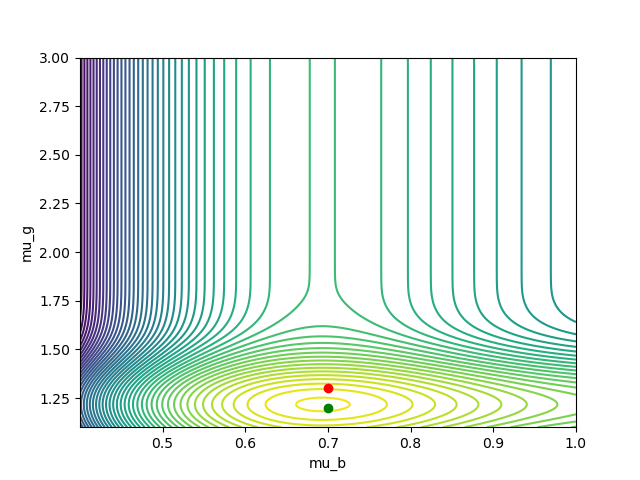
\includegraphics[width=.8\textwidth]{img/contour_mus.png}
  \caption{Contour plots of the likelihood versus means, for initial parameters 0.7, 1.3, 9.5, 0.1, 1 (that are considered easy, non problematic parameters). The red dot shows the parameters that generated the data, the green one the ones retrieved by the optimizer.}
  \label{fig:easy_par}
\end{figure}


\begin{figure}
  \centering
  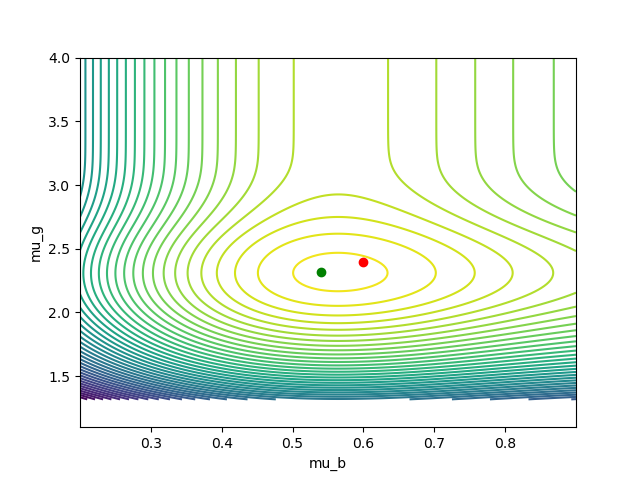
\includegraphics[width=.8\textwidth]{img/contour_mus_not_converging.png}
  \caption{Contour plots of the likelihood versus means, for initial parameters 0.6, 2.4, 10, 0.2, 1 (that are considered not easy, quite problematic parameters). The red dot shows the parameters that generated the data, the green one the ones retrieved by the optimizer.}
  \label{fig:diff_par}
\end{figure}


Figure~\ref{fig:easy_par} shows how the likelihood looks like plotted against the means of the parameters \(\beta\), \(\gamma\), and how the optimizer converges for easy parameters.
Figure \autoref{fig:diff_par} shows the same for more difficult parameters.

In both cases the sample size is 200 data points, and the plot is done fixing the other parameters (tha variances and the mean of \(t^*\)) to the original values, with which the data have been generated.

\begin{figure}
  \centering
  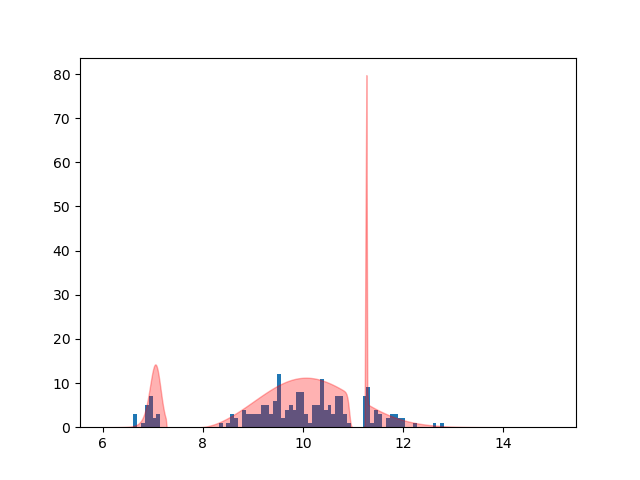
\includegraphics[width=.8\textwidth]{img/likelihood_over_ta}
  \caption{Plot of where the data actually are (in blue), versus where the data are forcasted to be knowing the actual parameters (in red). The sample size is 200 data points, and the parameters are, as earlier, 0.6, 2.4, 10, 0.2, 1}
  \label{fig:likelihood_over_tas}
\end{figure}

Lastly, figure~\autoref{fig:likelihood_over_tas} shows where, knowing the parameters but ithout knowing the data, the data are forcasted to be.
As can be seen, there is room for improvements in the location of the left spike. This is due to an error in estimating an integral that can be fixed.

\section{Modifying data}

Since some of the data we have regard the instantaneous travel time,
rather then the travel time given the arrival (or the departure) time,
it is necessary to transform the instantaneous travel time to the actual travel time necessary to travel through the bottleneck.

For computing the actual travel time, we suppose that the bottleneck has fixed length \(d^p\),
and that in each moment the instantaneous travel time \(v(t)\) is constant along it.
The length of the bottleneck will thus be

\begin{equation}
  \label{eq:len_bottleneck}
  d^p = \int_{t_i}^{t_f}v(t) dt
\end{equation}

Suppose thus \(v(t)\) has primitive \(V(t)\), such that

\begin{equation}
  \label{eq:primitive}
  \int_{t_i}^{t_f}v(t) dt = V(t_f) - V(t_i)
\end{equation}

Equation \eqref{eq:len_bottleneck} becomes trivially

\begin{align*}
  d^p & = V(t_f) - V(t_i) \\
  t_i & = V^{-1}(V(t_f) - d^p)
\end{align*}
and the travel time can thus be expressed in function of \(t_f\):

\begin{align*}
  \begin{split}
    \label{eq:travel_time}
    tt(t_f) & = t_i - t_f \\
    & = V^{-1}(V(t_f) - d^p) - t_f
  \end{split}
\end{align*}

In the case in which the instantaneous travel time increase linearly, its primitive is easy to compute and to invert:

\begin{align*}
  v(t) & = \bar{v}t \\
  V(t) & = \frac{\bar{v}}{2}t^2 \\
  V^{-1}(x) & = \sqrt{\frac{2x}{\bar{v}}}
\end{align*}
and thus,
\begin{align*}
  tt(t_f) & = \sqrt{\frac{2}{\bar{v}}\left(\frac{\bar{v}}{2}t_f^2 - d^p\right)} - t_f \\
  & = \sqrt{t_f^2 - \frac{2}{\bar{v}}d^p} - t_f
\end{align*}

\subsection{Numerically}

Numerically, it may be impossible (or very inconvenient) to find the actual primitive \(V(t)\).

An approach that can be taken (especially when the travel time function is just a discrete set of values) is to directly approximate the integral in \eqref{eq:len_bottleneck}.
This can be done by progressively increasing the domain of integration (where the integration is discrete, approximated with trapezoids),
until the integral becomes larger than the bottleneck length \(d^p\).

\begin{figure}
  \centering
  \makebox[\textwidth][c]{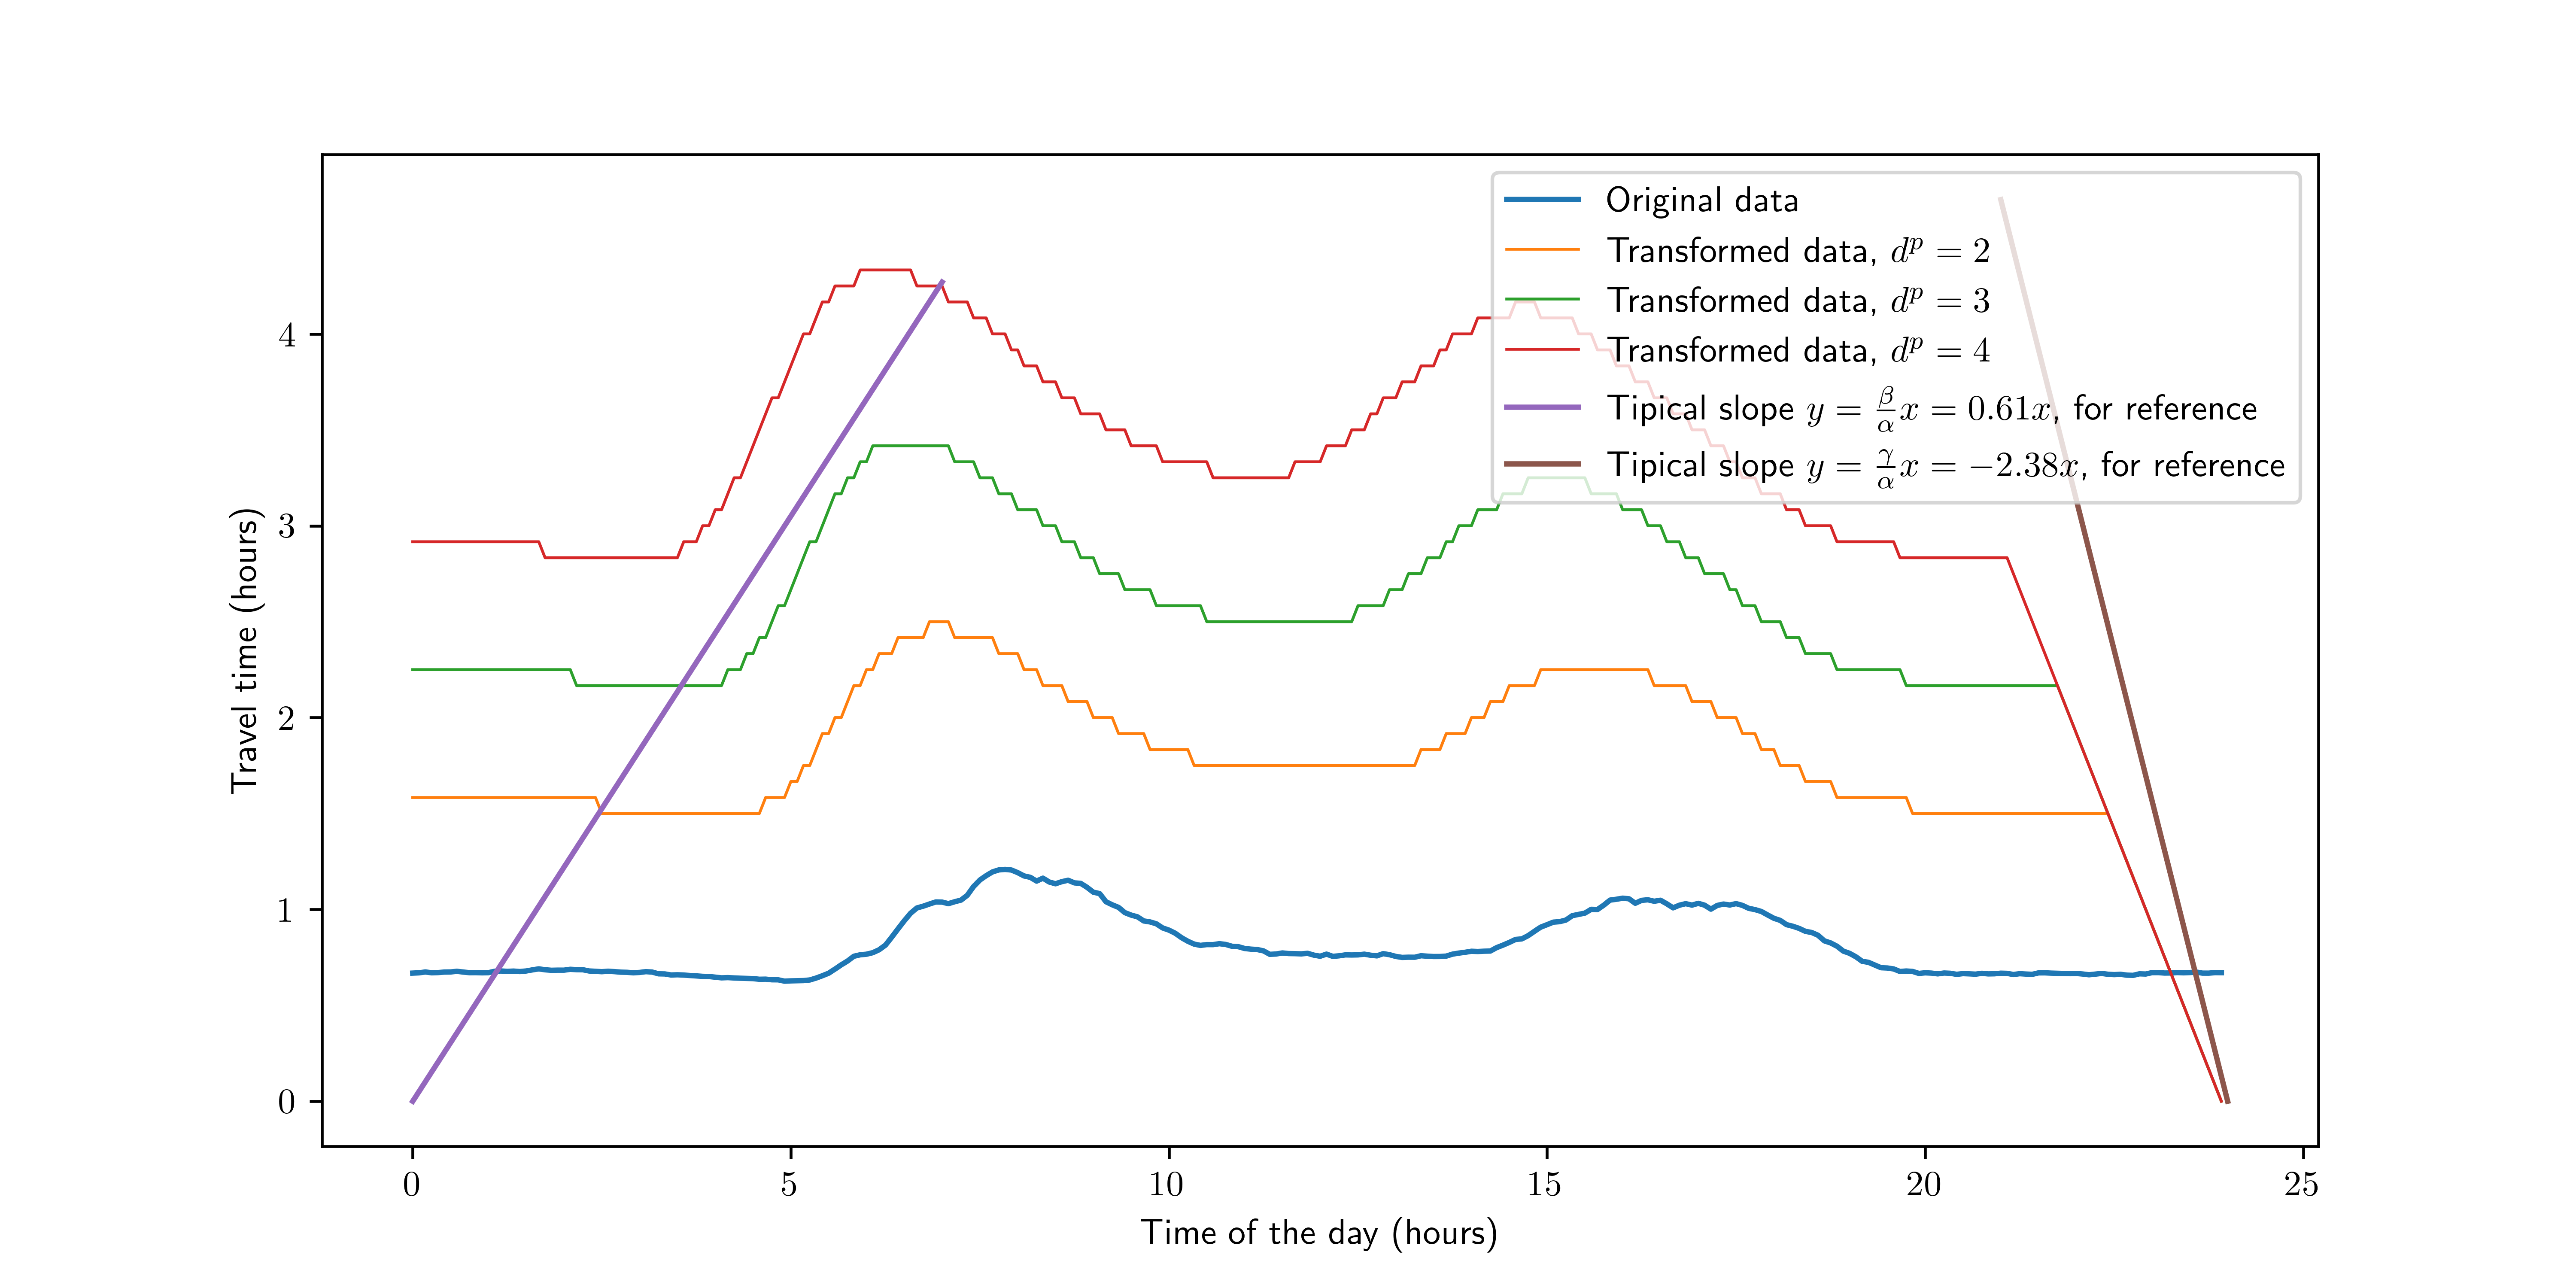
\includegraphics[width=1.9\textwidth]{img/transforming_data}}
  \caption{Transformed data, for different values of the bottleneck length $d^p$. The lines whose steepness yields late and early arrivals are shown for reference, in order to be able to appreciate the increasing steepness}
  \label{fig:modifying_data}
\end{figure}

Figure \ref{fig:modifying_data} shows the result of this process, for different values of the parameter \(d^p\).
Sadly, plotting the derivative is not particularly meaningful without smoothing the function beforehand,
since the function is piecewise constant.

\end{document}
%%% Local Variables:
%%% mode: LaTeX
%%% TeX-master: t
%%% End:
